\documentclass{article}
\usepackage{fullpage}
\usepackage{graphicx}
\graphicspath{ {images/} }
\author{Michael Miller}
\title{PA1 Report}

\begin{document}
\begin{description}

\item[Algorithm Description] Jacobi 1D represents the application of heat onto a discretized 1-dimensional rod, and how the temperature of the rod sections change over time. The code does this by allocating an array of user inputted size (i.e., generates the rod) then sets the values of the $0^{th}$ and $n^{th}$ elements to equal 5000 (i.e., applies the heat). The code, then, iterates through a loop (i.e., time passes) and sets the temperature of each segment of rod equal to the average of its own temperature, its left neighbor, and its right neighbor (i.e., allows heat to propagate throughout the rod).

Jacobi 2D works in the same way, but heat is applied on the perimeter of a 2D plane, and each array element is set equal to the average of its 9 neighbors.

Mat vec takes a vector and a matrix, naively multiplies them, and stores the result in a third vector.

\item[Description of Parallelization Approach] For Jacobi 1D, the code was parallelized on the \emph{for} loop, and a static schedule was used. Because of the regularity of this algorithm, a static schedule is appropriate, as all iterations take $\mathcal{O}(1)$ time. 

For Jacobi 2D, there are two options for simple parallelization: parallelizing the inner or outer loop. For contiguity, parallelizing the inner loop makes sense, as this will provide spatial locality. Although, in practice, parallelizing the inner loop causes too much parallelization overhead via fork/join calls. This leaves us with parallelizing the outer loop, which upon experimentation, yields a faster execution time for the same input. A static schedule was used for Jacobi 2D, for similar reasons as Jacobi 1D.

For mat vec, the outer \emph{for} loop was parallelized, using a static schedule, as every computation is $\mathcal{O}(1)$. In practice, static, dynamic (with a chunk size of 3125), and guided yield very similar results in terms of execution time. Perhaps this is because the tradeoffs between overhead and parallelization throughput are equal. A larger input size was attempted to ascertain which schedule would be faster, although a segfault was halting that experiment.

\item[Experimental Setup] The algorithms were tested on Montgomery, which has a cache size of 20480 KB per core, using 8 threads for parallel sections of the code. For all three algorithms, sequential execution times will be compared against parallel execution times (with the inclusion of static, dynamic, and guided schedules).

\item[Experimental Results] 
	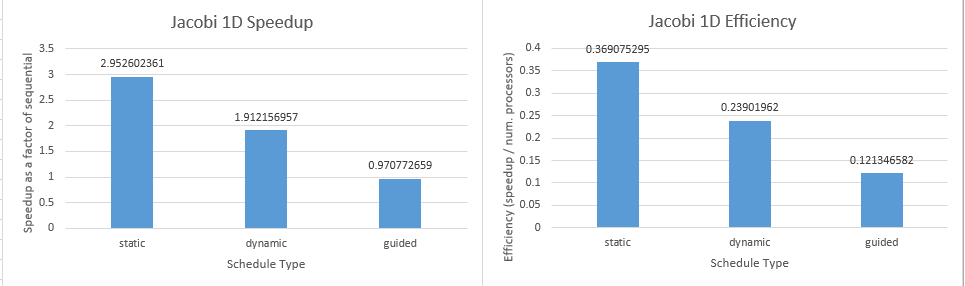
\includegraphics{jacobi}
	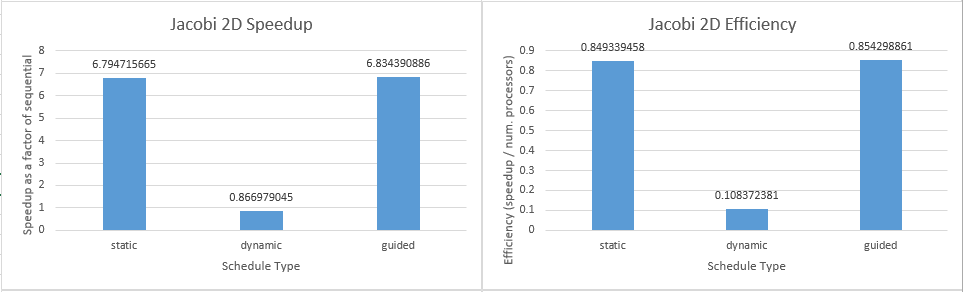
\includegraphics{jacobi2d}
	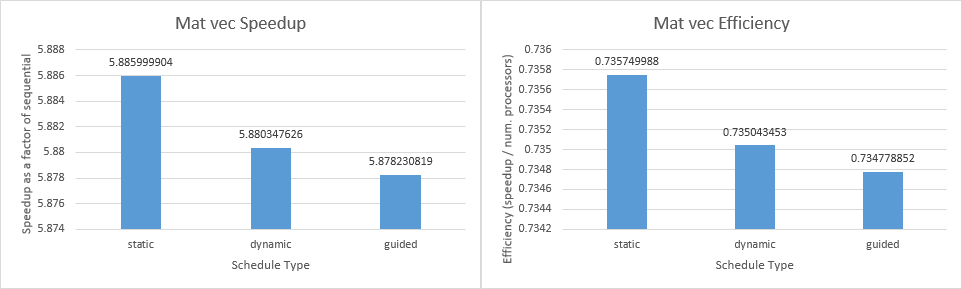
\includegraphics{mat_vec}
\end{description}
\end{document}
